\maketitle
\tableofcontents
\newpage

\section{Zielsetzung}
Ziel dieses Versuches ist es, das Relaxationsverhalten eines RC-Gliedes zu
untersuchen. Dabei wird die Zeitkonstante des Kreises bestimmt, die Amplitude
der Kondensatorspannung und die Phasenverschiebung zwischen Generator- und Kondensatorspannung
in Abhängigkeit von der Frequenz aufgenommen und ermittelt, unter welchen Vorraussetzungen
ein RC-Kreis als Integrator genutzt werden kann.
\section{Theorie}
\subsection{Relaxationserscheinungen ohne Periodizität}
Wenn ein System aus seinem Ausgangszustand entfernt wird und ihn nicht mittels Ozillation
wieder erreicht, dann spricht man von Relaxation. Dabei ist die Änderungsgeschwindigkeit
der Größe $A$ proportional zu
\begin{equation}
    \frac{\symup dA}{\symup dt} = c \left[A(t) - A(\infty) \right]
    \label{eqn:1}
\end{equation}
mit $t = bel.$ und $A(\infty)$ der Endzustand des Systems. Wenn \eqref{eqn:1} über
die Zeitpunkte 0 bis $t$ integriert wird, folgt
\begin{equation}
    A(t) = A(\infty) + \left[A(0) - A(\infty) \right] e^{\, ct} \, .
    \label{eqn:2}
\end{equation}
Damit \eqref{eqn:2} beschränkt bleibt, muss $c < 0$ gelten. Als Beispiel für
solche Relaxationsvorgänge lässt sich das Auf- und Entladen eines Kondensators
über einen Widerstand nennen. Eine passende Schaltung ist in Abbildung \ref{fig:1}
dargestellt.
\begin{figure}
  \centering
  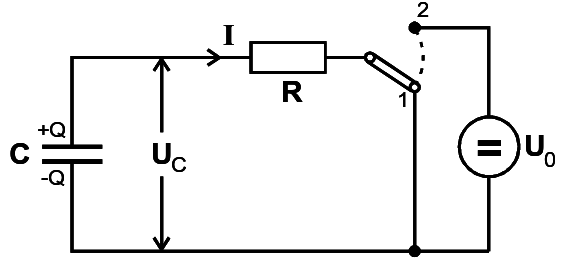
\includegraphics[scale=0.5]{kondensator.png}
  \caption{Schaltskizze zum Auf- (Stellung 2) und Entladen (Stellung 1) eines
  Kondensators \cite{anleitung}.}
  \label{fig:1}
\end{figure}
\begin{itemize}
  \item \textbf{Entladevorgang}:

  Es wird angenomen, dass zum Zeitpunkt $t = 0$ die Ladung $Q$ auf dem Kondensator
  mit der Kapazität $C$ liegt. Damit folgt für die Spannung
  \begin{equation*}
    U_\symup{C} = \frac{Q}{C} \, .
  \end{equation*}
  Unter Zuhilfenahme des ohmschen Gesetztes und der Beziehung zwischen zeitlicher Änderung
  deR Ladung in Relation zum Strom ergibt sich eine Differentialgleichung nach Gestalt
  von \eqref{eqn:1}. Wenn man annimmt, dass nach unendlicher langer Zeit der Kondensator vollständig
  entladen ist, und ersetzt in \eqref{eqn:2} $U(\infty)$ mit 0, dann folgt
  \begin{equation}
    Q(t) = Q(0) e^{-\frac{t}{RC}} \, .
    \label{eqn:3}
  \end{equation}

  \item \textbf{Aufladevorgang}:

  Nach dem gleichen Prinzip erfolgt die Aufladung eines Kondensators; diesmal mit
  den Randbedingungen
  \begin{align*}
      Q(0) &= 0 \\
      Q(\infty) &= C U_0 \, .
  \end{align*}
  Damit folgt eine Gleichung ähnlich zu \eqref{eqn:3} nach Gestalt von \eqref{eqn:2}
  \begin{equation}
    Q(t) = C U_0 \left(1 - e^{-\frac{t}{RC}} \right) \, ,
    \label{eqn:4}
  \end{equation}
  wobei der Ausdruck $RC$ als Zeitkonstante bezeichnet wird. Diese Zeitkonstante
  liefert eiine Aussage über die Geschwindigkeit mit der der Endzustand erreicht wird.
\end{itemize}

\subsection{Relaxationserscheinungen mit Periodizität und RC-Glied als Integrator}
Relaxationsvorgänge treten auch auf, wenn das System periodisch ausgelenkt wird. Um
dies zu untersuchen, wird der Schaltplan aus Abbildung \ref{fig:1} nun um einen
Wechselstromgenerator erweitert, der eine sinusförmige Spannung mit
\begin{equation}
    U(t) = U_0 \, \symup{cos} \left(\omega t \right)
    \label{eqn:5}
\end{equation}
liefert. Ein solcher Schaltplan ist in Abbildung \ref{fig:2} zu sehen.
\begin{figure}
  \centering
  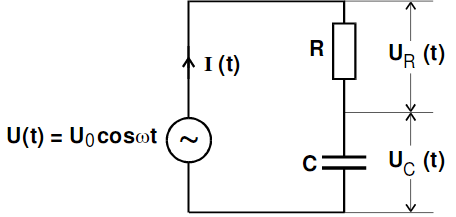
\includegraphics[scale=0.6]{kondensator2.png}
  \caption{Schaltskizze zur Untersuchung von Relaxationserscheinungen bei
  periodischen Auslenkungen. \cite{anleitung}}
  \label{fig:2}
\end{figure}
Solange in \eqref{eqn:5} $\omega << 1/(RC)$ gilt, kann man annehmen, dass die Spannung
am Kondensator zu jeder Zeit praktisch gleich $U(t)$ ist. Wenn nun $\omega$ größer
wird, dann wird sich eine Phase $\phi$ zwischen Kondensator- und Generatorspannung
bilden und die Amplitude $A$ der Kondensatorspannung wird sinken. Zur weiteren
Untersuchung des Phänomens lässt sich mit dem Ansatz
\begin{equation}
    U_\symup{C}(t) = A(\omega) \, \symup{cos} \left[\omega t + \phi (\omega)  \right]
    \label{eqn:6}
\end{equation}
ein Ausdruck für die Frequenzanhängigkeit der Phase
\begin{equation}
  \phi (\omega) = \symup{arctan} \left(- \omega RC \right)
  \label{eqn:7}
\end{equation}
finden. An \eqref{eqn:7} lässt sich bestätigen, dass die Phasenverschiebung für
kleine $\omega$ gegen 0 und für große gegen $\frac{\pi}{2}$ geht. Für die Amplitude
$A$ in Abhängigkeit von der Frequenz ergibt sich
\begin{equation}
    A(\omega) = \frac{U_0}{\sqrt{1 + \omega^2 R^2 C^2}} \, .
    \label{eqn:8}
\end{equation}
Die Amplitude $A(\omega)$ geht für $\omega \to 0$ gegen $U_0$ und für
$\omega \to \infty$ gegen 0; so wie bereits diskutiert. Aus diesem Grund wird
ein RC-Kreis oft als Tiefpass verwendet.

Unter der Vorraussetzung, dass $\omega$ gegenüber $\frac{1}{RC}$ viel größer ist,
kann ein RC-Glied auch die angelegte Spannung $U(t)$ integrieren. In diesem Fall
gilt näherungsweise
\begin{equation}
    U_\symup{C} (t) = \frac{1}{RC} \int_0^t U(t') \symup d t' \, .
    \label{eqn:9}
\end{equation}

\section{Durchführung}

\subsection{Versuchsaufbau}

\subsection{Versuchsdurchführung}

\section{Auswertung}

\section{Diskussion}
\newpage
\nocite{*}
\printbibliography
